\documentclass[12pt]{article}
\usepackage{amsmath}
\usepackage{hyperref}
\usepackage{graphicx}
\usepackage{fullpage}
\title{A Pita-Form With No Crease}
\author{Alex Cole and Ben Kraft}
\begin{document}
\maketitle

\section{The problem:}
In \textit{Generalized D-Forms Have No Spurious Creases}, Eric Demaine and Gregory Price show that all of the creases in the flat components of a seam form (a convex surface that is flat everywhere except finitely many smooth curves) occur between vertices or are tangent to the seams. As a corallary, this implies that pita-forms (or seam forms made from a sewing a single smooth convex shape along its boundary) must have only 1 crease though the flat region that runs between the 2 vertices (the start and end points of the sewing). Up until now, all examples of pita-forms have exhibited this crease, but at \url{http://gfalop.org/closed.open}, it was asked whether pita-forms always have this crease. Here we demonstrate a pita-form with no crease.

\section{Our construction}
Our surface is created by taking the convex hull of a unit spring of height $h$. So we look at the curve traced by the parametric equation 
$$(x(t), y(t), z(t)) = \left(1-\cos(2\pi t), \sin(2\pi t), ht \right) \text{ for } t \in [0, 1]$$
and take the convex hull. Letting $h=5$ and approximating the curve with 150 points, we get something that looks like:

\begin{center}
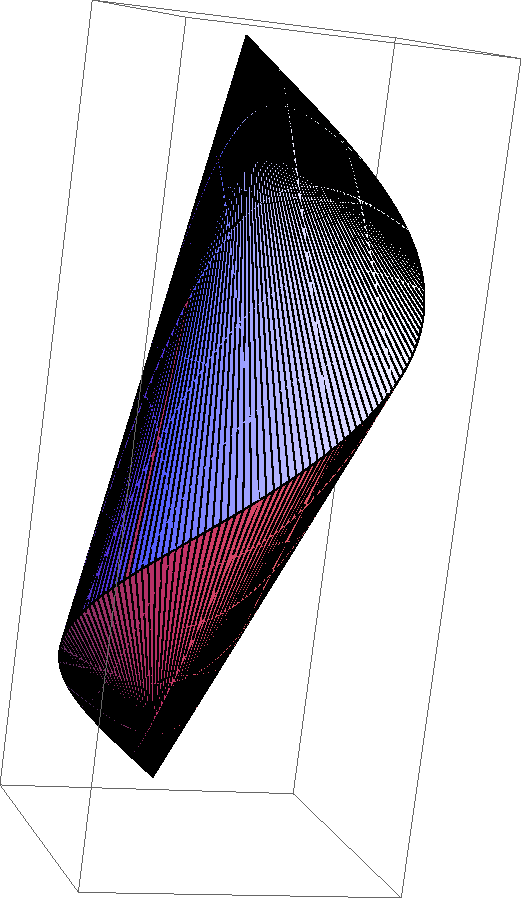
\includegraphics[scale=.6]{pita_h=5_n=150.pdf}
\end{center}

\subsection{Is it a pita form?}
This is a natural first question to ask about the surface. 

First, note that every point of the parametric equation is actually on the surface and furthermore, the segment running from each point of the coil to each of the 2 vertices is on the surface, so the entire surface is ruled and therefore flat. This is fairly clear when you look at the 50 point approximation below:
\begin{center}
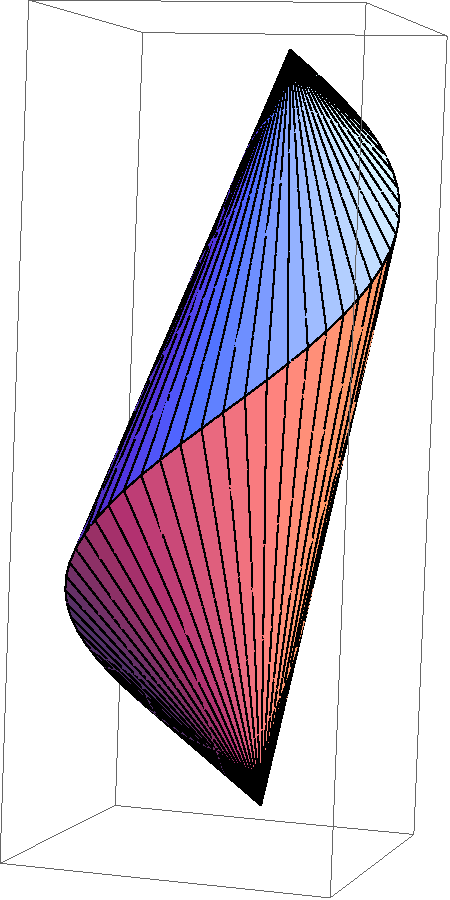
\includegraphics[scale=.6]{pita_h=5_n=50.pdf}
\end{center}

Now that we know that it is flat, we can flatten it out to check that it comes from a smooth convex shape. To do that, we will look at just one half of the figure (split by the line between the vertices) and come up with a polar parametric equation for it. We will use the same 1 parameter $t$ that runs from 0 to 1 and turn it into a flattened polar parametric system by keeping track of the distance to the start point (origin) for $r(t)$ and looking at the accumulated angle $\theta (t)$. 

Let's start with $r(t)$. For this we can just use the Pythagorean theorem to find the distance from the point on the sew line of our pita form at  $(x(t), y(t), z(t)) = \left(1-\cos(2\pi t), \sin(2\pi t), ht \right)$ to $(0,0,1)$. Doing this we get:

$$ r(t) = \sqrt{h^2(t-1)^2+ \sin (2\pi t)^2+ (1-\cos(2\pi t))^2}$$

Now for $\theta(t)$ we can just find an expression for $d\theta$ and then integrate it along the curve. At any time $t$ we can form a triangle with vertices $(0, 0, 0), (x(t), y(t), z(t)),$ and $(x(t+dt), y(t+dt), z(t+dt))$. The angle at the origin is $d\theta$ and the 2 sides adjacent to that have lengths $r(t)$ and $r(t+dt)$. The remaining side has length $\sqrt{4 \pi^2 +h^2}dt$ because our original parametric curve has length $\sqrt{4 \pi^2 +h^2}$ and moves at a constant speed.

So using law of cosines:
$$\left(\sqrt{4 \pi^2 +h^2}dt\right)^2 = r(t)^2 + r(t+dt)^2 - 2r(t)r(t+dt)\cos ( d\theta)$$

Now using a 2nd order Taylor approximation for the cosine:

$$\left(\sqrt{4 \pi^2 +h^2}dt\right)^2 = r(t)^2 + r(t+dt)^2 - 2r(t)r(t+dt)\left(1- \frac{d\theta^2}{2}\right)$$

$$(4 \pi^2 +h^2)dt^2 = (r(t) - r(t+dt))^2 +r(t)r(t+dt)d\theta^2$$


$$4 \pi^2 +h^2= \left(\frac{r(t) - r(t+dt)}{dt}\right)^2 +r(t)r(t+dt)\left(\frac{d\theta}{dt}\right)^2$$

$$4 \pi^2 +h^2= r'(t)^2 +r(t)^2\left(\frac{d\theta}{dt}\right)^2$$

$$\frac{d\theta}{dt} = \frac{\sqrt{h^2 + 4 \pi^2 - r'(t)^2}}{r(t)} $$

$$\theta(t) = \int_0^t \frac{\sqrt{h^2 + 4 \pi^2 - r'(s)^2}}{r(s)} ds$$

Now to show that it is a pita form, we need to check that it comes from a smooth convex shape. To examine this we can look at the unfoldings for $h=3$, 5, and 7:
\begin{center}
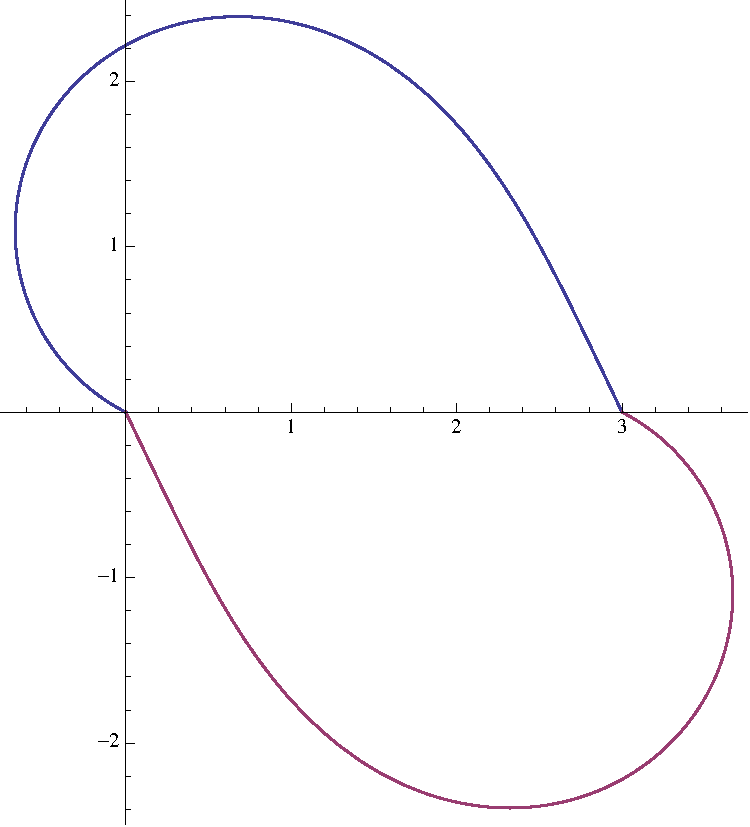
\includegraphics[scale=.4]{unfold_h=3.pdf}
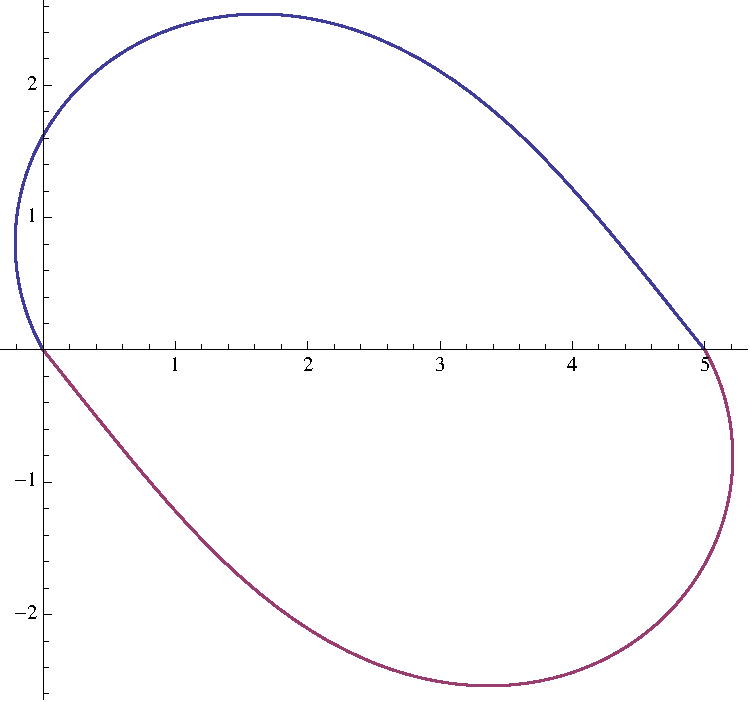
\includegraphics[scale=.4]{unfold_h=5.pdf}
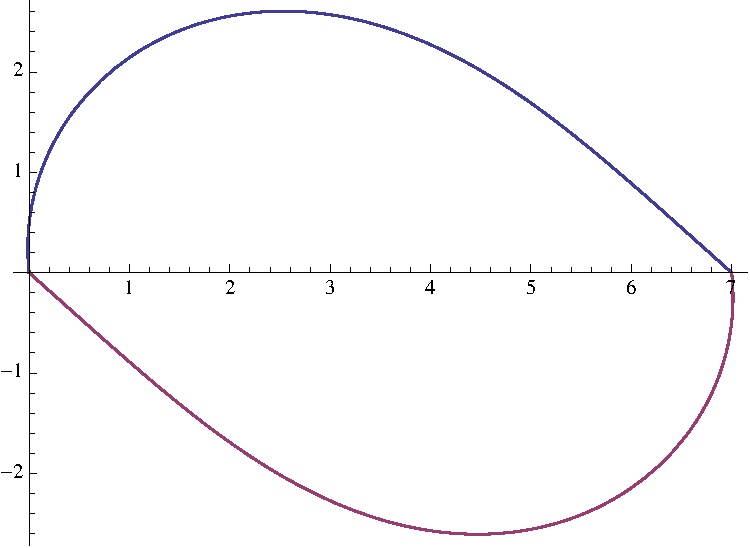
\includegraphics[scale=.4]{unfold_h=7.pdf}
\end{center}

The angle at the origin is then $\theta_0(h)=\theta(1)+\tan^{-1}\left(\frac{2\pi}{h}\right)$.  In particular, $\theta(1)$ is the portion of the angle above the $x$-axis; the curve intersects the origin at $t=1$.  The other portion of the angle can be found by looking at the 3D pita-form; it is the angle between the line between the two vertices, and the curve.  Because one of the bounding lines is vertical, the surface is locally vertical, so the angle will remain unchanged if we imagine our surface going downwards (in the negative $z$ direction) everywhere. This means that our modified surface is just a right triangle cuved in a cylindrical fashion. The triangle has a base of $2\pi$ and height $h$, so this portion of the angle is $\arctan \frac{2\pi}{h}$.

This is decreasing in $h$, and can be computed to be more than $180^\circ$ at for example $h=3$ and less than $180^\circ$ at $h=7$.  Then since the angle is a continuous function of $h$, there is some $h^*$ in between 3 and 7 such that there is exactly $180^\circ$ of material around each vertex causing the shape to be smooth.  We may then solve numerically for $h^*$:

$$ \theta_0(h^*)= 180^\circ= \theta(1)+\arctan \frac{2\pi}{h^*}$$
$$h^*\approx 4.55199394344572$$

So our final smooth unfolding with $h=h^*$ looks like
\begin{center}
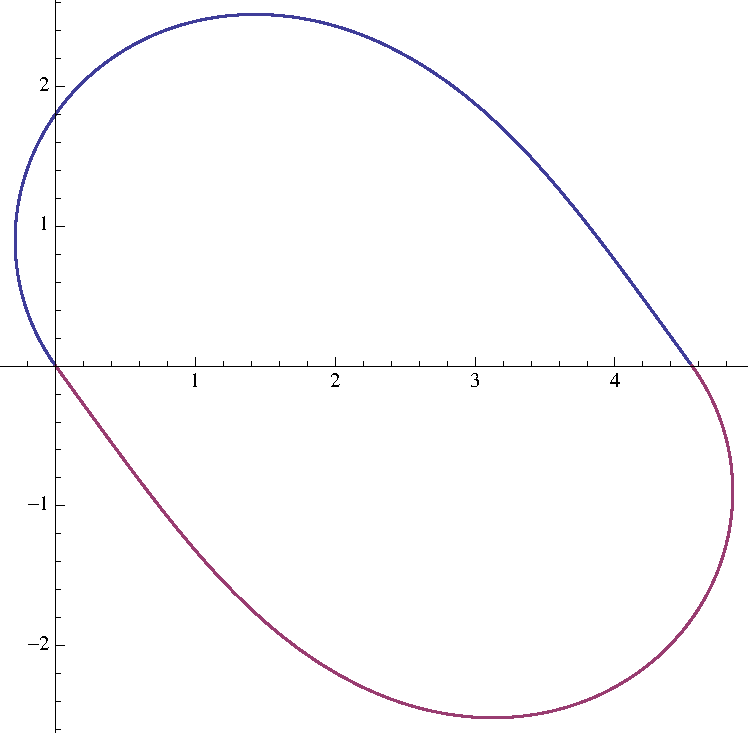
\includegraphics[scale=.4]{unfold_h=h*.pdf}
\end{center}

\subsection{Is there a crease?}
Getting back to our original question, did we actually construct a pita form without a crease?
\begin{center}
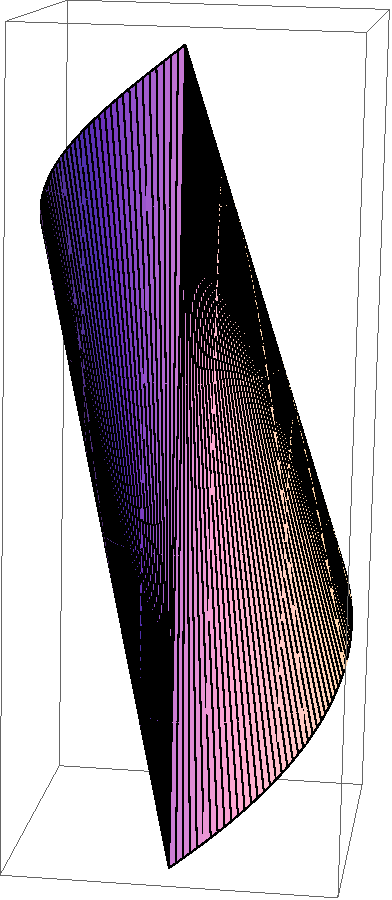
\includegraphics[scale=.6]{crease_h=5_n=150.pdf}
\end{center}
Assume that there is a crease. Then it must be between the 2 vertices of our pita-form. Also if it is a crease, then there is an infinite family of tangent planes tangent to the pita-form along the crease. But our original parametric curve lies along a cylinder of radius 1 along the $z$-axis. So looking at our tangent plane, we see that it must also be tangent to this cylinder and the cylinder is smooth, so there is only 1 tangent plane to each vertical segment on the surface. This means that there is a unique tangent plane to the crease, so it isn't a crease at all. 

This means that this is in fact a pita-form with no crease. Woo hoo!

\end{document}